\documentclass[11pt]{article}

\usepackage{amsmath,amssymb}
\usepackage{amsthm}
\usepackage{graphicx}
\usepackage{booktabs}
\usepackage{hyperref}
\usepackage{geometry}
\usepackage{algorithm}
\usepackage{algpseudocode}
\usepackage{caption}
\usepackage{subcaption}
\usepackage{tikz}
\usepackage{pgfplots}
\usepackage{pgfplotstable}
\usepackage{placeins}
\usepackage{float}
\pgfplotsset{compat=1.18}

% Path to benchmark data (different for article vs SEA version)
\newcommand{\rootdir}{.}

% Load benchmark metadata from CSV
\pgfplotstableread[col sep=comma]{\rootdir/figures/rust/metadata.csv}\rustmetadata
\pgfplotstablegetelem{0}{value}\of\rustmetadata \let\rustbenchmarkdate\pgfplotsretval
\pgfplotstablegetelem{1}{value}\of\rustmetadata \let\rustbenchmarkmachine\pgfplotsretval
\pgfplotstablegetelem{2}{value}\of\rustmetadata \let\rustbenchmarkn\pgfplotsretval
\pgfplotstablegetelem{3}{value}\of\rustmetadata \let\rustbenchmarkiterations\pgfplotsretval

% Command to add benchmark note to figures
\newcommand{\rustbenchmarknote}{\par\vspace{2pt}\noindent{\scriptsize\textit{Benchmarked on \rustbenchmarkmachine\ (\rustbenchmarkdate), $n=\rustbenchmarkn$, \rustbenchmarkiterations\ iterations.}}}
\usetikzlibrary{positioning,arrows.meta,patterns,calc,decorations.pathreplacing,pgfplots.fillbetween}

\geometry{margin=1in}

% Theorem environments
\newtheorem{theorem}{Theorem}
\newtheorem{lemma}[theorem]{Lemma}
\newtheorem{corollary}[theorem]{Corollary}
\newtheorem{proposition}[theorem]{Proposition}
\theoremstyle{definition}
\newtheorem{definition}[theorem]{Definition}
\newtheorem{example}[theorem]{Example}
\theoremstyle{remark}
\newtheorem{remark}[theorem]{Remark}
\newtheorem{claim}[theorem]{Claim}

\title{DeltaSort: Incremental repair of sorted arrays with known updates}
\author{Shubham Dwivedi \\
\small Independent Researcher \\
\small \texttt{shubd3@gmail.com}
}
\date{2026}

\begin{document}
\maketitle

\begin{abstract}
Reading sorted data is a fundamental requirement in almost all data processing systems. When dealing with large sorted datasets that require great read performance, sorting-on-read is not feasible. A standard approach is to have a derived sorted read-replica that is updated with the latest snapshot asynchronously whenever the system-of-record gets updated. For updating read-replicas, most production systems resort to either full re-sorting or Binary-Insertion-Sort or Extract-Sort-Merge. In this paper, we show that these traditional approaches can be significantly improved for certain workloads. This paper also formulates an alternative model in which the sorting routine is explicitly informed of the updated indices since the previous sort. Under this model, we present \emph{DeltaSort}, an efficient incremental repair algorithm for arrays. We present experimental evidence that shows that \emph{DeltaSort} outperforms existing approaches for a wide range of update batch sizes for our Rust implementation. These results suggest that tighter integration between update pipelines and sorting routines can yield significant performance gains in real incremental-sorting workloads. We also explore limitations of this approach and identify a clear crossover point, depending on array size, where full re-sorting becomes preferable. 
\end{abstract}

%==============================================================================
\section{Introduction}
%==============================================================================

Sorting is among the most optimized primitives in modern systems, backed by decades of deep research. Standard library implementations---TimSort~\cite{timsort}, Introsort~\cite{musser1997introspective}, and PDQSort~\cite{peters2021pdqsort} deliver excellent performance for general inputs by exploiting partial order, cache locality, and adaptive strategies. However, these algorithms operate under a \emph{blind} model: they discover structure dynamically rather than being explicitly informed about which values have changed since the previous sort.

In many practical systems, this assumption is unnecessarily pessimistic. Sorted arrays are often maintained incrementally in read-heavy workloads where updates affect only a subset of values and the indices of those updates can be easily tracked if needed. Nevertheless, this information is typically not tracked or utilized, and systems fall back to blind re-sorting or standard repair approaches using Binary-Insertion-Sort or Extract-Sort-Merge. As an example, consider a web application that shows a real-time game leaderboard. Being able to efficiently update the sorted view on updates directly impacts the user experience. The traditional approaches fall short---full re-sort can block the main UI thread for long durations, while Binary-Insertion-Sort can be slow for a large number of updates. To address these limitations, this paper makes the following contributions:

\begin{enumerate}
  \item \textbf{Update-aware sorting model:}
  We formulate an incremental sorting model in which the sorting routine is explicitly informed of the updated indices since the previous sort. Under this model, Binary-Insertion-Sort and Extract-Sort-Merge serve as natural baseline algorithms for maintaining sorted order through incremental updates.

  \item \textbf{DeltaSort algorithm:}
  We present \emph{DeltaSort}, an incremental repair algorithm for sorted arrays designed for the update-aware model. DeltaSort batches multiple updates and achieves multi-fold speedups over traditional approaches for a wide range of update batch sizes.
\end{enumerate}

%==============================================================================
\section{Related Work}
\label{sec:related}
%==============================================================================

%TODO: Talk about parallelizable sorting algorithms

Adaptive sorting algorithms exploit existing order in the input to improve performance on nearly sorted data. TimSort~\cite{timsort} and natural merge sort~\cite{knuth1998art} dynamically identify monotonic runs and merge them efficiently, while a substantial body of work formalizes measures of presortedness and analyzes sorting complexity as a function of these measures rather than input size alone~\cite{mannila1985measures}. These approaches, however, operate under a blind model: partial order must be rediscovered through full-array scans, and no external information about which values have changed is assumed.

A separate line of work studies incremental computation and view maintenance in database and streaming systems, where changes to input data are propagated to derived results using explicit delta representations~\cite{gupta1995maintenance, nikolic2014incremental, akidau2015dataflow}. These techniques focus on maintaining query results, aggregates, and materialized views, and operate at the level of relational or dataflow operators rather than array-based sorting primitives. While they demonstrate the practical value of update-aware computation, they do not specifically address the problem of efficiently restoring sorted order in arrays under batched point updates.

Dynamic data structures offer a different trade-off. Self-balancing trees such as AVL trees~\cite{avl1962}, red--black trees~\cite{guibas1978dichromatic}, B-trees~\cite{bayer1972organization}, and skip lists~\cite{pugh1990skip} support efficient ordered updates with logarithmic cost, but abandon contiguous array layout and its attendant cache locality. Library sort~\cite{bender2004insertion} reduces insertion overhead by maintaining gaps within arrays, but addresses online insertion and incurs additional space overhead.

In contrast, this work considers maintaining sorted order in arrays where the indices of updated values since the previous sort are explicitly available. \emph{DeltaSort} performs segmented repair without auxiliary data structures, which distinguishes it from prior adaptive sorting algorithms, incremental view maintenance techniques, and dynamic ordered data structures.

%==============================================================================
\section{Problem Model}
\label{sec:model}
%==============================================================================

\begin{definition}[Update-Aware Sorting]
\label{def:problem}
Let $A[0..n-1]$ be an array sorted according to a strict weak ordering defined by a comparator $\texttt{cmp}$. Let $U = \langle u_1, u_2, \dots, u_k \rangle$ be a sequence of indices such that \[ 0 \le u_1 < u_2 < \dots < u_k \le n-1, \] and the values at these indices may have been arbitrarily updated, while values at all other indices remain unchanged. The \emph{update-aware sorting problem} is to restore $A$ to a state that is sorted with respect to $\texttt{cmp}$, given explicit knowledge of the set $U$.
\end{definition}

%==============================================================================
\section{DeltaSort Algorithm}
\label{sec:algorithm}
%==============================================================================

\subsection{Overview}

\begin{definition}[Violation]
\label{def:violation}
For an updated index $i$, we classify its \emph{violation} based on local order:
\begin{itemize}
  \item \textbf{LEFT (L)}: Value \textbf{must} move left---$\texttt{cmp}(A[i-1], A[i]) > 0$ (for $i > 0$).
  \item \textbf{RIGHT (R)}: Value \textbf{may} move right and \textbf{cannot} move left.
\end{itemize}
\end{definition}

Every updated index is either a LEFT or RIGHT violation. Violation is only defined for updated indices and has no meaning for clean indices.

\begin{definition}[Segment]
\label{def:segment}
A \emph{segment} is a \textbf{maximal subarray} of $U$ whose values follow the pattern $(\mathrm{R})^*(\mathrm{L}^+ \mid \epsilon)$: zero or more RIGHT violations followed by one or more LEFT violations, or end of array. Figure~\ref{fig:segment-structure} illustrates this structure.
\end{definition}

% Figure: Segment structure diagram
\begin{figure}[H]
\centering
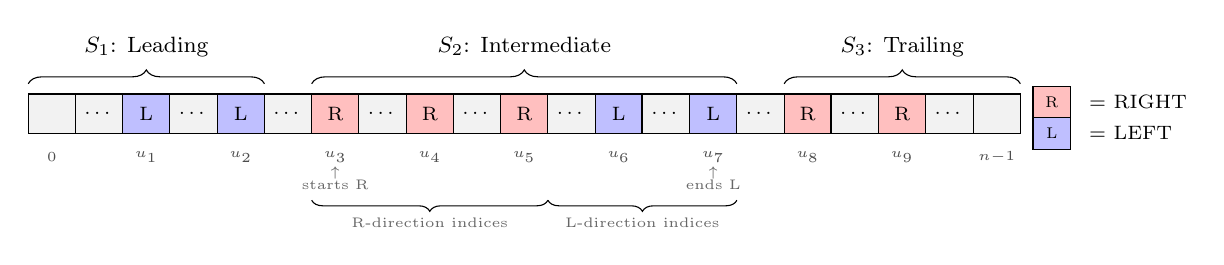
\begin{tikzpicture}[
    cell/.style={minimum width=0.6cm, minimum height=0.5cm, draw, font=\scriptsize},
    dotcell/.style={minimum width=0.5cm, minimum height=0.5cm, font=\scriptsize},
    indexcell/.style={minimum width=0.6cm, font=\tiny, text=black!70},
    right/.style={cell, fill=red!25},
    left/.style={cell, fill=blue!25},
    clean/.style={cell, fill=gray!10, font=\scriptsize},
    segbrace/.style={decorate, decoration={brace, amplitude=5pt}},
    segbracem/.style={decorate, decoration={brace, amplitude=4pt, mirror}},
    seglabel/.style={font=\footnotesize},
    condlabel/.style={font=\tiny, text=black!60},
    faded/.style={opacity=0.4}
]

% Array indices (shown below)
\def\yidx{-0.55}
\def\yarr{0}

% === ARRAY START ===
\node[clean] at (-0.9, \yarr) {};
\node[indexcell] at (-0.9, \yidx) {$0$};
\node[clean] at (-0.3, \yarr) {\dots};

% === LEADING SEGMENT (L's only, bounded by array start) ===
\node[left] (l0) at (0.3, \yarr) {L};
\node[indexcell] at (0.3, \yidx) {$u_1$};
\node[clean] at (0.9, \yarr) {\dots};
\node[left] (l1) at (1.5, \yarr) {L};
\node[indexcell] at (1.5, \yidx) {$u_2$};

% Inter-segment clean region
\node[clean] at (2.1, \yarr) {\dots};

% === MIDDLE SEGMENT (R's then L's) ===
\node[right] (r1) at (2.7, \yarr) {R};
\node[indexcell] at (2.7, \yidx) {$u_3$};
\node[clean] at (3.3, \yarr) {\dots};
\node[right] (r2) at (3.9, \yarr) {R};
\node[indexcell] at (3.9, \yidx) {$u_4$};
\node[clean] at (4.5, \yarr) {\dots};
\node[right] (r3) at (5.1, \yarr) {R};
\node[indexcell] at (5.1, \yidx) {$u_5$};
\node[clean] at (5.7, \yarr) {\dots};
\node[left] (l2) at (6.3, \yarr) {L};
\node[indexcell] at (6.3, \yidx) {$u_6$};
\node[clean] at (6.9, \yarr) {\dots};
\node[left] (l3) at (7.5, \yarr) {L};
\node[indexcell] at (7.5, \yidx) {$u_7$};

% Inter-segment clean region
\node[clean] at (8.1, \yarr) {\dots};

% === TRAILING SEGMENT (R's only, bounded by array end) ===
\node[right] (r4) at (8.7, \yarr) {R};
\node[indexcell] at (8.7, \yidx) {$u_8$};
\node[clean] at (9.3, \yarr) {\dots};
\node[right] (r5) at (9.9, \yarr) {R};
\node[indexcell] at (9.9, \yidx) {$u_9$};

% === ARRAY END ===
\node[clean] at (10.5, \yarr) {\dots};
\node[clean] at (11.1, \yarr) {};
\node[indexcell] at (11.1, \yidx) {$n{-}1$};

% === SEGMENT BRACES (top) ===
% Leading segment
\draw[segbrace] (-1.2, 0.38) -- (1.8, 0.38);
\node[seglabel] at (0.3, 0.85) {$S_1$: Leading};

% Middle segment
\draw[segbrace] (2.4, 0.38) -- (7.8, 0.38);
\node[seglabel] at (5.1, 0.85) {$S_2$: Intermediate};

% Trailing segment
\draw[segbrace] (8.4, 0.38) -- (11.4, 0.38);
\node[seglabel] at (9.9, 0.85) {$S_3$: Trailing};

% === SUB-BRACES for middle segment (bottom) ===
\draw[segbracem] (2.4, -1.1) -- (5.4, -1.1);
\node[condlabel, anchor=north] at (3.9, -1.2) {R-direction indices};
\draw[segbracem] (5.4, -1.1) -- (7.8, -1.1);
\node[condlabel, anchor=north] at (6.6, -1.2) {L-direction indices};

% === ANNOTATIONS for boundary conditions ===
% Condition markers (centered on cells)
\node[condlabel] at (2.7, -0.75) {$\uparrow$};
\node[condlabel] at (2.7, -0.9) {starts R};

\node[condlabel] at (7.5, -0.75) {$\uparrow$};
\node[condlabel] at (7.5, -0.9) {ends L};

% === LEGEND ===
\node[right, scale=0.8] at (11.8, 0.15) {R};
\node[font=\scriptsize, anchor=west] at (12.15, 0.15) {= RIGHT};
\node[left, scale=0.8] at (11.8, -0.25) {L};
\node[font=\scriptsize, anchor=west] at (12.15, -0.25) {= LEFT};

\end{tikzpicture}
\caption{A segment $(i,j)$ starts at either index $0$ or an R-direction updated index, and ends at either index $n{-}1$ or an L-direction updated index, with all R's preceding all L's within. In this example, the leading segment $S_1$ contains only L's (starting from index $0$), the intermediate segment $S_2$ contains R's followed by L's, and the trailing segment $S_3$ contains only R's (ending at index $n{-}1$). Leading and trailing segments may or may not be present depending on the directions of updated indices.}
\label{fig:segment-structure}
\end{figure}

DeltaSort operates in two phases:

\begin{enumerate}
  \item \textbf{Phase 1 (Segment):} Extract updated values, sort them, and write back to updated indices in index order. This establishes segments in the array that are disjoint and can be repaired independently.
  \item \textbf{Phase 2 (Repair):} Repair each segment left-to-right, deferring RIGHT indices to a stack until the first LEFT index is encountered. When a LEFT is encountered, first flush and repair all pending RIGHTs in LIFO order, then repair the LEFT. Continue left-to-right.
\end{enumerate}

Figure~\ref{fig:delta-sort-example} illustrates the full DeltaSort process on a small example.

% Example figure showing segmentation with concrete array
\begin{figure}[t]
\centering
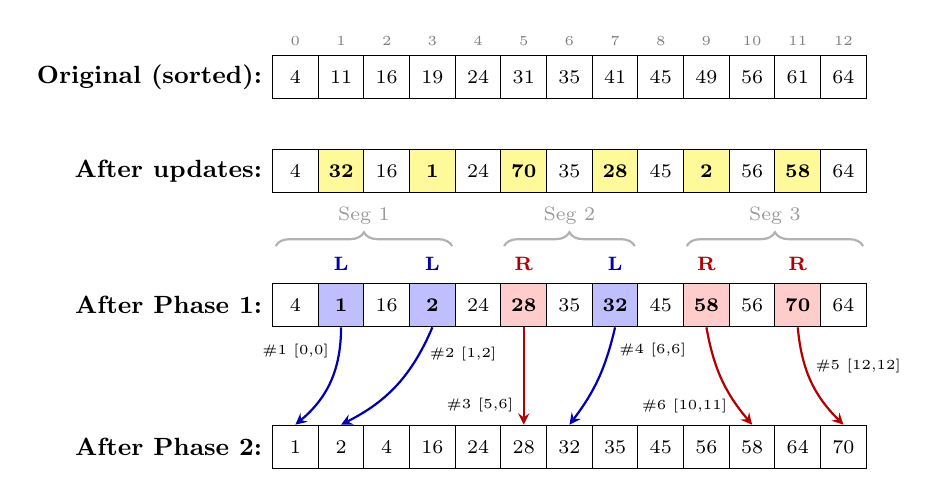
\begin{tikzpicture}[
    cell/.style={draw, minimum width=0.58cm, minimum height=0.55cm, font=\scriptsize},
    cellup/.style={cell, fill=yellow!40, font=\scriptsize\bfseries},
    cellL/.style={cell, fill=blue!25, font=\scriptsize\bfseries},
    cellR/.style={cell, fill=red!20, font=\scriptsize\bfseries},
    larrow/.style={->, >=stealth, thick, blue!70!black},
    rarrow/.style={->, >=stealth, thick, red!70!black},
    segbrace/.style={decorate, decoration={brace, amplitude=5pt}},
]

% === STAGE 1: Original sorted array ===
\node[font=\small\bfseries, anchor=east] at (-0.3, 0) {Original (sorted):};
\foreach \i/\v in {0/4, 1/11, 2/16, 3/19, 4/24, 5/31, 6/35, 7/41, 8/45, 9/49, 10/56, 11/61, 12/64} {
    \node[cell] (o\i) at (\i*0.58, 0) {\v};
}
% Index labels
\foreach \i in {0,...,12} {
    \node[font=\tiny, gray] at (\i*0.58, 0.45) {\i};
}

% === STAGE 2: After updates applied ===
\node[font=\small\bfseries, anchor=east] at (-0.3, -1.2) {After updates:};
\foreach \i/\v/\up in {0/4/0, 1/32/1, 2/16/0, 3/1/1, 4/24/0, 5/70/1, 6/35/0, 7/28/1, 8/45/0, 9/2/1, 10/56/0, 11/58/1, 12/64/0} {
    \ifnum\up=1
        \node[cellup] (u\i) at (\i*0.58, -1.2) {\v};
    \else
        \node[cell] (u\i) at (\i*0.58, -1.2) {\v};
    \fi
}

% === STAGE 3: After Phase 1 (sorted updates, L/R classified) ===
\node[font=\small\bfseries, anchor=east] at (-0.3, -2.9) {After Phase 1:};

% Segment braces (between Stage 2 and L/R labels)
\draw[segbrace, thick, gray!60] (0*0.58-0.25, -2.15) -- (3*0.58+0.25, -2.15) 
    node[midway, above=4pt, font=\scriptsize, gray!80] {Seg 1};
\draw[segbrace, thick, gray!60] (5*0.58-0.25, -2.15) -- (7*0.58+0.25, -2.15) 
    node[midway, above=4pt, font=\scriptsize, gray!80] {Seg 2};
\draw[segbrace, thick, gray!60] (9*0.58-0.25, -2.15) -- (12*0.58+0.25, -2.15) 
    node[midway, above=4pt, font=\scriptsize, gray!80] {Seg 3};

% L/R labels (just above Phase 1 array)
\node[font=\scriptsize, blue!70!black] at (1*0.58, -2.38) {\textbf{L}};
\node[font=\scriptsize, blue!70!black] at (3*0.58, -2.38) {\textbf{L}};
\node[font=\scriptsize, red!70!black] at (5*0.58, -2.38) {\textbf{R}};
\node[font=\scriptsize, blue!70!black] at (7*0.58, -2.38) {\textbf{L}};
\node[font=\scriptsize, red!70!black] at (9*0.58, -2.38) {\textbf{R}};
\node[font=\scriptsize, red!70!black] at (11*0.58, -2.38) {\textbf{R}};

% Phase 1 array: 4, 1, 16, 2, 24, 28, 35, 32, 45, 58, 56, 70, 64
% Only color violation cells (L=blue, R=red), others plain
\node[cell] (p0) at (0*0.58, -2.9) {4};
\node[cellL] (p1) at (1*0.58, -2.9) {1};
\node[cell] (p2) at (2*0.58, -2.9) {16};
\node[cellL] (p3) at (3*0.58, -2.9) {2};
\node[cell] (p4) at (4*0.58, -2.9) {24};
\node[cellR] (p5) at (5*0.58, -2.9) {28};
\node[cell] (p6) at (6*0.58, -2.9) {35};
\node[cellL] (p7) at (7*0.58, -2.9) {32};
\node[cell] (p8) at (8*0.58, -2.9) {45};
\node[cellR] (p9) at (9*0.58, -2.9) {58};
\node[cell] (p10) at (10*0.58, -2.9) {56};
\node[cellR] (p11) at (11*0.58, -2.9) {70};
\node[cell] (p12) at (12*0.58, -2.9) {64};

% === STAGE 4: After Phase 2 (fully sorted) ===
\node[font=\small\bfseries, anchor=east] at (-0.3, -4.7) {After Phase 2:};

% Final sorted: 1, 2, 4, 16, 24, 28, 32, 35, 45, 56, 58, 64, 70
\foreach \i/\v in {0/1, 1/2, 2/4, 3/16, 4/24, 5/28, 6/32, 7/35, 8/45, 9/56, 10/58, 11/64, 12/70} {
    \node[cell] (f\i) at (\i*0.58, -4.7) {\v};
}

% Movement arrows from Phase 1 to Phase 2 (updated values only)
% Labels show: #fix_number (leftBound, rightBound) - placed beside arrows
\draw[larrow, bend left=25] (p1.south) to node[font=\tiny, black, left, pos=0.2] {\#1 [0,0]} (f0.north);
\draw[larrow, bend left=20] (p3.south) to node[font=\tiny, black, right, pos=0.2] {\#2 [1,2]} (f1.north);
\draw[rarrow] (p5.south) to node[font=\tiny, black, left, pos=0.8] {\#3 [5,6]} (f5.north);
\draw[larrow, bend left=12] (p7.south) to node[font=\tiny, black, right, pos=0.2] {\#4 [6,6]} (f6.north);
\draw[rarrow, bend right=15] (p9.south) to node[font=\tiny, black, left, pos=0.8] {\#6 [10,11]} (f10.north);
\draw[rarrow, bend right=20] (p11.south) to node[font=\tiny, black, right, pos=0.35] {\#5 [12,12]} (f12.north);

\end{tikzpicture}
\caption{Segmentation example: An array of size 13 with 6 updates at indices 1, 3, 5, 7, 9, 11. 
In \textbf{Phase~1}, updated values are sorted among themselves and written back to the array. Each value is classified as \textcolor{blue!70!black}{L} or \textcolor{red!70!black}{R}.
In \textbf{Phase~2}, each value is fixed one by one. The label numbers indicate the fixing order, along with the computed left and right bounds for binary search for each updated value.}
\label{fig:delta-sort-example}
\end{figure}

\subsection{Key Insight: \emph{Segmentation enables localized repair}}
\label{sec:insight}

The key insight behind DeltaSort is that pre-sorting updated values induces a \emph{segmentation} of updates. After Phase~1, updated indices partition into disjoint segments of the form $(\mathrm{R})^*(\mathrm{L}^+ \mid \epsilon)$.

\begin{lemma}[Movement Confinement]
\label{lem:confinement}
Value movement during the repair phase is bounded within each segment: no value needs to cross a segment boundary.
\end{lemma}

\begin{proof}
Let $S$ be a segment with RIGHT indices $R_1, \ldots, R_m$ followed by LEFT indices $L_1, \ldots, L_p$ (where $m \ge 0$ and $p \ge 0$, with $m + p \ge 1$). After Phase~1, updated values are monotonically ordered by index, so $A[R_1] < \cdots < A[R_m] < A[L_1] < \cdots < A[L_p]$.

\begin{enumerate}
  \item RIGHT values move rightward but cannot pass the first LEFT index $L_1$ (if it exists) or the segment boundary, since $A[R_i] < A[L_1]$ for all $i$.

  \item LEFT values move leftward but cannot pass the last RIGHT index $R_m$ (if it exists) or the segment boundary, since $A[R_m] < A[L_j]$ for all $j$.
\end{enumerate}

Since no value exits its segment, each segment can be repaired independently. The more segments we have after Phase~1, more localized fixes are possible. Theorem~\ref{thm:movement-bound} establishes an asymptotic bound on number of segments.
\end{proof}

\subsection{Pseudocode}

\begin{algorithm}[H]
\caption{DeltaSort}
\label{alg:deltasort}
\begin{algorithmic}[1]
\Require Array $A[0..n-1]$, updated indices $U$, comparator $\texttt{cmp}$
\Ensure $A$ is sorted
\Statex
\State \textbf{Phase 1: Establish segments}
\State $\texttt{updatedIndices} \gets \text{sort}(U)$;
\State $\texttt{updatedValues} \gets \text{sort}([A[u] : u \in \texttt{updatedIndices}], \texttt{cmp})$
\For{$i \gets 0$ \textbf{to} $|\texttt{updatedIndices}| - 1$}
\State $A[\texttt{updatedIndices}[i]] \gets \texttt{updatedValues}[i]$
\EndFor
\State $\texttt{updatedIndices.push}(n)$; \Comment{Sentinel for handling trailing segment with no LEFT's}
\Statex
\State \textbf{Phase 2: Fix segments}
\State $\texttt{pendingRight} \gets []$; $\texttt{leftBound} \gets 0$
\For{$p \gets 0$ \textbf{to} $|\texttt{updatedIndices}| - 1$}
    \State $i \gets \texttt{updatedIndices}[p]$; $\texttt{dir} \gets (i = n)$ ? \textsc{Left} : $\Call{GetDirection}{A, i}$
    \If{$\texttt{dir} = \textsc{Left}$}
        \State $\texttt{rightBound} \gets i - 1$
        \While{$\texttt{pendingRight} \neq \emptyset$}
            \State $j \gets \texttt{pendingRight.pop}()$
            \If{$\texttt{cmp}(A[j], A[j+1]) > 0$}
                \State $\texttt{rightBound} \gets \Call{FixRight}{A, j, \texttt{rightBound}} - 1$
            \EndIf
        \EndWhile
        \If{$i < n$} \Comment{Skip dummy LEFT sentinel}
            \State $\texttt{leftBound} \gets \Call{FixLeft}{A, i, \texttt{leftBound}} + 1$
        \EndIf
    \Else
        \State $\texttt{pendingRight.push}(i)$ \Comment{Defer RIGHT violation}
    \EndIf
\EndFor
\end{algorithmic}
\end{algorithm}

\vspace{0.5em}

\noindent\begin{minipage}{\linewidth}
\begin{algorithmic}[1]
\Function{GetDirection}{$A$, $i$}
    \State \Return $i > 0 \land \texttt{cmp}(A[i-1], A[i]) > 0$ ? \textsc{Left} : \textsc{Right}
\EndFunction
\end{algorithmic}
\end{minipage}

\vspace{0.5em}

\noindent\begin{minipage}{\linewidth}
\begin{algorithmic}[1]
\Function{FixLeft}{$A$, $i$, $\texttt{leftBound}$}
    \State $t \gets \Call{BinarySearchLeft}{A, A[i], \texttt{leftBound}, i-1}$
    \State \Call{Move}{A, i, t}
    \State \Return $t$
\EndFunction
\end{algorithmic}
\end{minipage}

\vspace{0.5em}

\noindent\begin{minipage}{\linewidth}
\begin{algorithmic}[1]
\Function{FixRight}{$A$, $i$, $\texttt{rightBound}$}
    \State $t \gets \Call{BinarySearchRight}{A, A[i], i+1, \texttt{rightBound}}$
    \State \Call{Move}{A, i, t};
    \State \Return $t$
\EndFunction
\end{algorithmic}
\end{minipage}

\subsection{Correctness Proof}

\begin{lemma}[Violation Fix Invariant]
\label{lem:fix-invariant}
Each fix operation during Phase~2 resolves a violation without introducing new ones.
\end{lemma}

\begin{proof}
We fix each violation using binary search. For binary search to find the correct insertion point, the search range must contain no violations.

\begin{itemize}
    \item \emph{LEFT fix at index $i$}: The search range $[leftBound, i-1]$ contains no LEFT violations because LEFTs are processed left-to-right, and no RIGHT violations because all pending RIGHTs are flushed before any LEFT is fixed.
    \item \emph{RIGHT fix at index $i$}: The search range $[i+1, rightBound]$ contains no RIGHT violations because RIGHTs are processed in LIFO order with $rightBound$ narrowing after each fix, and no LEFT violations because $rightBound$ never extends past the first LEFT in the segment.
\end{itemize}

\end{proof}

\begin{theorem}[Correctness]
\label{thm:correctness}
DeltaSort produces a correctly sorted array.
\end{theorem}

\begin{proof}
The only violations in the array after Phase~1 are at updated indices. Phase~2 processes each updated index exactly once. By Lemma~\ref{lem:fix-invariant}, each fix resolves a violation without introducing new ones. After all fixes, no violations remain, so the array is sorted.
\end{proof}

\subsection{Complexity Analysis}
% TODO: Establish 2 class of algorithms: blind vs update-aware and clearly call out with algorithms belong where

\begin{theorem}[Asymptotic Movement Bound]
\label{thm:movement-bound}
The total number of movements for repairing $k$ udpdated indices in an array of size $n$ using DeltaSort is $\theta(n)$.
\end{theorem}

\begin{proof}
  WIP
\end{proof}

\begin{theorem}[Time Complexity]
\label{thm:time}
DeltaSort runs in $O(k \log k + k \log n + M)$ time, where $M$ is the total movement.
\end{theorem}

\begin{proof}
We analyze the two phases separately.

\paragraph{Phase 1.}
Sorting the $k$ updated indices and their corresponding values costs $O(k \log k)$ time.
Writing the sorted values back requires $O(k)$ time.

\paragraph{Phase 2.}
Each updated index is processed once. Violation checks cost $O(1)$ per index, and each repair performs a binary search over a sorted region in $O(\log n)$ time. Thus Phase~2 requires $O(k \log n)$ time. Let $M$ denote the total number of values moved during repair. The movement cost is $O(M)$.

\paragraph{Total.}
The overall complexity is $O(k \log k + k \log n + M)$.
\end{proof}

\begin{theorem}[Space Complexity]
\label{thm:space}
DeltaSort uses $O(k)$ auxiliary space.
\end{theorem}

\begin{proof}
Phase~1 stores $k$ updated indices and $k$ updated values. Phase~2 maintains a pending stack of at most $k$ indices. No $O(n)$ auxiliary structures are required.
\end{proof}

\begin{remark}[Movement Efficiency]
While worst-case movement is $O(kn)$, the segmentation created by Phase~1 tends to reduce movement in the average case. Empirical results in \S\ref{sec:experiments} demonstrate substantial speedups, validating that segmentation (Lemma~\ref{lem:confinement}) effectively reduces movement in practice. We will analyze average-case movement more rigorously in future work.
\end{remark}

Table~\ref{tab:complexity} compares algorithm complexity with the standard baseline approaches used in the experiments:
\begin{itemize}
  \item \textbf{NativeSort (NS)}: Re-sort the array using the natively available sort function. $O(n \log n)$ comparisons and movements.
  \item \textbf{Binary-Insertion-Sort (BIS)}: Extract updated values, then for each: binary search for correct position, reinsert. $O(k \log n)$ comparisons, $O(kn)$ worst-case movement. Searches the full array range for each insertion.
  \item \textbf{Extract-Sort-Merge (ESM)}: Extract updated values, sort them, merge with clean values. $O(k \log k + n)$ comparisons, $O(n)$ movement. Requires $O(n)$ auxiliary space.
\end{itemize}

\begin{table}[t]
\centering
\caption{Algorithm complexity comparison}
\label{tab:complexity}
\begin{tabular}{l c c c c}
\toprule
Algorithm & Comparisons (C) & Movement (M) & Space (S) & Time (C + M) \\
\midrule
FullSort$^{*}$ $(\texttt{sort\_by})$ & $O(n \log n)$ & - & - & $O(n \log n)$ \\
BIS & $O(k \log n)$ & $O(kn)$ & $O(1)$ & $O(kn)$ \\
ESM & $O(k \log k + n)$ & $O(n)$ & $O(n)$ & $O(k \log k + n)$ \\
\textbf{DeltaSort} & $O(k \log n)$ & $O(n\sqrt{k})$ & $O(k)$ & $O(k \log n + n \sqrt k)$$^{\dagger}$ \\
\bottomrule
\end{tabular}

\vspace{0.3em}
{\small $^{*}$Not update-aware; hence complexity is a function of only $n$. The exact movement and space complexity are implementation-dependent and not required for the present discussion.}


{\small $^{\dagger}$Expected. Worst-case time is $O(kn)$}
\end{table}

%==============================================================================
\section{Experimental Evaluation}
\label{sec:experiments}
%==============================================================================


All experiments are run using a Rust implementation of DeltaSort~\cite{deltasort-repo} on a synthetic dataset of user objects with composite keys (country, age, name) on an M3 Pro MacBook Pro with 18GB RAM. Each data point is the mean of 20--1000 iterations (more iterations for small $k$ to account for timer resolution). Coefficient of variation was below 15\% for all measurements; raw data with confidence intervals is available in the repository.

\subsection{Algorithms Compared}

DeltaSort is compared against four baselines:
\begin{itemize}
    \item \textbf{NativeSort}: Rust's \texttt{sort\_by} (PDQSort~\cite{peters2021pdqsort}), representing the standard approach of re-sorting the entire array. Used as baseline for execution time.
    \item \textbf{MergeSort}: A standard merge sort implementation, included to provide an instrumentable blind-sort baseline for data movement measurements (NativeSort's internal movements cannot be directly tracked).
    \item \textbf{Binary-Insertion-Sort (BIS)}: The naive incremental approach---extract updated values, then reinsert each using binary search. $O(k \log n)$ comparisons but $O(kn)$ movements.
    \item \textbf{Extract-Sort-Merge (ESM)}: Extract updated values, sort them separately, and merge with the remaining sorted portion. $O(k \log k + n)$ comparisons and $O(n)$ movements.
\end{itemize}

\subsection{Correctness}
Correctness is formally proven in Theorem~\ref{thm:correctness} and also verified by an extensive set of randomized unit tests~\cite{deltasort-repo} across various scales and update sizes. The test routine generates a sorted base array of size $n$, applies $k$ random updates at random indices, runs DeltaSort, and asserts that the final array is sorted and contains all original values with updated values. All tests pass successfully.

\subsection{Execution Time}

Figure~\ref{fig:rust-execution-time} shows execution time (in microseconds) for $n = 50$K values as a function of updated count $k$. DeltaSort consistently outperforms all alternatives up to approximately $k = 16.5$K (crossover point), achieving significant speedups of $4$--$20\times$ over NativeSort in the intermediate range. Also note the orders-of-magnitude gap between DeltaSort and the baseline incremental algorithms (BIS and ESM) across the full range of $k$ values.

% Figure: All algorithms comparison (log-log scale)
\begin{figure}[H]
\centering
\begin{tikzpicture}
\begin{axis}[
    width=0.8\textwidth,
    height=5cm,
    xlabel={Number of updated values ($k$)},
    ylabel={Execution time (\textmu s)},
    xmode=log,
    ymode=log,
    log basis x=10,
    log basis y=10,
    xmin=1, xmax=100000,
    ymin=5, ymax=100000,
    xtick={1, 10, 100, 1000, 10000, 100000},
    xticklabels={1, 10 (0.01\%), 100 (0.1\%), 1K (1\%), 10K (10\%), 100K},
    legend pos=south east,
    legend style={font=\small, fill=white, fill opacity=0.95, draw=gray!50},
    grid=major,
    major grid style={line width=0.3pt, draw=gray!30},
    tick label style={font=\small},
    label style={font=\small},
]

% FullSort
\addplot[color=gray!70, mark=square*, thick, mark size=2pt] 
    table[col sep=comma, x=k, y=native] {\rootdir/figures/js/execution-time.csv};

% Binary Insertion
\addplot[color=orange!80, mark=triangle*, thick, mark size=2pt] 
    table[col sep=comma, x=k, y=bis] {\rootdir/figures/js/execution-time.csv};
% Extract-Sort-Merge
\addplot[color=purple!70, mark=diamond*, thick, mark size=2pt] 
    table[col sep=comma, x=k, y=esm] {\rootdir/figures/js/execution-time.csv};

% DeltaSort (emphasized)
\addplot[color=green!70!black, mark=*, thick, mark size=2.5pt, line width=1.5pt] 
    table[col sep=comma, x=k, y=deltasort] {\rootdir/figures/js/execution-time.csv};

\legend{FullSort, BIS, ESM, \textbf{DeltaSort}}
\end{axis}
\end{tikzpicture}
\caption{Execution time comparison for JavaScript implementations for $n = 100$K (log-log scale).}
\label{fig:js-execution-time}
\end{figure}


\subsection{Comparator Invocation Count}

Figure~\ref{fig:rust-comparator-count} shows the number of comparator invocations for each algorithm. DeltaSort and BIS both achieve $O(k \log n)$ comparisons, substantially fewer than NativeSort's $O(n \log n)$ and ESM's $O(k \log k + n)$. The comparison counts for DeltaSort are 10--40\% higher than BIS, indicating that DeltaSort's performance advantage comes from reduced data movement (Lemma~\ref{lem:confinement}). This also suggests that in scenarios with expensive comparators, the speedups from \emph{DeltaSort} over NativeSort may be even greater.

% Figure: Comparator invocation count comparison
\begin{figure}[H]
\centering
\begin{tikzpicture}
\begin{axis}[
    width=0.92\textwidth,
    height=6cm,
    xlabel={Number of updated values ($k$)},
    ylabel={Comparator invocations},
    xmode=log,
    ymode=log,
    log basis x=10,
    log basis y=10,
    xmin=1, xmax=100000,
    ymin=10, ymax=10000000,
    xtick={1, 10, 100, 1000, 10000},
    xticklabels={1, 10, 100, 1K, 10K},
    ytick={10, 100, 1000, 10000, 100000, 1000000, 10000000},
    yticklabels={10, 100, 1K, 10K, 100K, 1M, 10M},
    legend pos=south east,
    legend style={font=\small},
    grid=both,
    grid style={line width=0.1pt, draw=gray!30},
    major grid style={line width=0.2pt, draw=gray!50},
]

% Native Sort
\addplot[color=gray!70, mark=square*, thick, mark size=2.5pt] 
    table[col sep=comma, x=k, y=native] {\rootdir/figures/rust/comparator-count.csv};

% Binary Insertion
\addplot[color=orange!80, mark=triangle*, thick, mark size=2.5pt] 
    table[col sep=comma, x=k, y=bis] {\rootdir/figures/rust/comparator-count.csv};

% Extract-Sort-Merge
\addplot[color=purple!70, mark=diamond*, thick, mark size=2.5pt] 
    table[col sep=comma, x=k, y=esm] {\rootdir/figures/rust/comparator-count.csv};

% DeltaSort (emphasized)
\addplot[color=green!70!black, mark=*, thick, mark size=2.5pt, line width=1.5pt] 
    table[col sep=comma, x=k, y=deltasort] {\rootdir/figures/rust/comparator-count.csv};

\legend{NativeSort, BIS, ESM, \textbf{DeltaSort}}
\end{axis}
\end{tikzpicture}
\caption{Comparator invocation count for $n = 50$K. DeltaSort and BIS
both achieve $O(k \log n)$ comparisons, while NativeSort uses $O(n \log n)$ regardless
of $k$, and ESM uses $O(k \log k + n)$. The 10--40\% higher comparison counts for DeltaSort
vs BIS confirm that movement confinement (Lemma~\ref{lem:confinement}) is the major factor in DeltaSort speedup.\rustbenchmarknote}
\label{fig:rust-comparator-count}
\end{figure}


\subsection{Data Movement Count}

Figure~\ref{fig:rust-movement-count} shows the number of data movements (element writes) for each algorithm. MergeSort provides an instrumented baseline for blind sorting with $O(n \log n)$ movements. BIS exhibits the highest movement count due to its $O(kn)$ complexity from repeated insertions. ESM requires $O(n)$ movements for the final merge. DeltaSort achieves 2--3 orders of magnitude fewer movements than all alternatives for small $k$, confirming that Lemma~\ref{lem:confinement}'s confinement guarantee translates to practical efficiency gains.

% Figure: Data movement count comparison (log-log scale)
\begin{figure}[H]
\centering
\begin{tikzpicture}
\begin{axis}[
    width=0.92\textwidth,
    height=7.5cm,
    xlabel={Number of updated values ($k$)},
    ylabel={Data movements (count)},
    xmode=log,
    ymode=log,
    log basis x=10,
    log basis y=10,
    xmin=1, xmax=30000,
    ymin=1000, ymax=1000000000,
    xtick={1, 10, 100, 1000, 10000},
    xticklabels={1, 10, 100, 1K, 10K},
    legend pos=north west,
    legend style={font=\small, fill=white, fill opacity=0.95, draw=gray!50},
    grid=major,
    major grid style={line width=0.3pt, draw=gray!30},
    tick label style={font=\small},
    label style={font=\small},
]

% MergeSort (instrumented baseline for blind sort)
\addplot[color=gray!70, mark=square*, thick, mark size=2pt] 
    table[col sep=comma, x=k, y=mergesort] {\rootdir/figures/rust/movement-count.csv};

% Binary Insertion
\addplot[color=orange!80, mark=triangle*, thick, mark size=2pt] 
    table[col sep=comma, x=k, y=bis] {\rootdir/figures/rust/movement-count.csv};

% Extract-Sort-Merge
\addplot[color=purple!70, mark=diamond*, thick, mark size=2pt] 
    table[col sep=comma, x=k, y=esm] {\rootdir/figures/rust/movement-count.csv};

% DeltaSort (emphasized)
\addplot[color=green!70!black, mark=*, thick, mark size=2.5pt, line width=1.5pt] 
    table[col sep=comma, x=k, y=deltasort] {\rootdir/figures/rust/movement-count.csv};

\legend{MergeSort, BIS, ESM, \textbf{DeltaSort}}
\end{axis}
\end{tikzpicture}
\caption{Data movement comparison for $n = 50$K (log-log scale). MergeSort provides an instrumented baseline for blind sorting ($O(n \log n)$ movements). DeltaSort achieves 2--3 orders of magnitude fewer movements than both MergeSort and the incremental algorithms for small $k$.\rustbenchmarknote}
\label{fig:rust-movement-count}
\end{figure}


\subsection{Crossover Threshold Analysis}

A key practical question is: at what update count should one switch from DeltaSort to NativeSort? A binary search was conducted for the crossover point $k_c$ across array sizes from 1K to 10M values.

Figure~\ref{fig:rust-crossover-threshold} visualizes how the crossover ratio $k_c / n$ varies with array size. The ratio peaks around ${\sim}33\%$ for medium-sized arrays ($n \approx 50$K) and declines rapidly for very large arrays ($n > 500$K), suggesting that DeltaSort's advantage narrows as arrays grow very large. This could be because the segmentation does not grow linearly with array size and hence advantages diminish at larger scales. More study is needed to understand this trend fully.

% Figure: Crossover ratio vs array size
\begin{figure}[H]
\centering
\begin{tikzpicture}
\begin{axis}[
    width=0.92\textwidth,
    height=6.5cm,
    xlabel={Array size ($n$)},
    ylabel={Crossover ratio $k_c / n$ (\%)},
    xmode=log,
    log basis x=10,
    xmin=500, xmax=20000000,
    ymin=0, ymax=40,
    ytick={0, 10, 20, 30, 40},
    yticklabels={0, 10, 20, 30, 40},
    xtick={1000, 10000, 100000, 1000000, 10000000},
    xticklabels={1K, 10K, 100K, 1M, 10M},
    legend pos=north east,
    legend style={font=\small, fill=white, fill opacity=0.95, draw=gray!50},
    grid=both,
    grid style={line width=0.1pt, draw=gray!20},
    major grid style={line width=0.2pt, draw=gray!40},
    tick label style={font=\small},
    label style={font=\small},
]

% Shaded region below the curve (DeltaSort wins)
\addplot[name path=curve, color=blue!70!black, mark=*, thick, mark size=2.5pt, line width=1.2pt] table[col sep=comma, x index=0, y index=1] {\rootdir/figures/rust/crossover-threshold.csv};
\path[name path=bottom] (axis cs:1000,0) -- (axis cs:10000000,0);
\addplot[green!20, opacity=0.5] fill between[of=curve and bottom];

% Vertical line at n=50K (the case evaluated in execution time chart)
\draw[purple!70!black, thick, dashed] (axis cs:50000, 0) -- (axis cs:50000, 40);
\node[circle, fill=purple!70!black, inner sep=3pt] at (axis cs:50000, 33.4) {};
\node[font=\scriptsize\bfseries, text=purple!70!black, anchor=south west] at (axis cs:55000, 34) {$n{=}50$K (Fig.~\ref{fig:rust-execution-time})};

% Annotation for the region
\node[font=\footnotesize, text=green!50!black] at (axis cs:5000, 12) {DeltaSort faster};

\end{axis}

% Benchmark metadata (right margin, rotated)
\end{tikzpicture}
\caption{Crossover ratio $k_c / n$ as a function of array size. DeltaSort outperforms NativeSort when the updated fraction is below the curve (shaded region).\rustbenchmarknote}
\label{fig:rust-crossover-threshold}
\end{figure}

The key takeaway is that DeltaSort offers the best incremental sort performance for \textbf{large} ranges of update sizes (0--30\% for the dataset we tested). The exact crossover threshold depends on the specific scenario (array size, data types, comparator cost, etc.).

\subsection{Performance in managed execution environments}

DeltaSort was also implemented in JavaScript~\cite{deltasort-repo} and benchmarked on the V8 engine to evaluate behavior in managed runtimes. Initial results indicate that DeltaSort outperforms NativeSort for some workloads, but the gains are more modest and the crossover point occurs at smaller update sizes. This behavior appears to be driven primarily by the performance characteristics of the native JavaScript sort, which is highly optimized and handles nearly sorted inputs exceptionally well. As a result, the relative advantage of segmented repair is reduced in this environment compared to the Rust implementation. The JavaScript benchmarks are still being refined and will be reported in a later revision. Until then, the Rust implementation provides the primary and authoritative performance characterization.

%==============================================================================
\section{Future Work}
\label{sec:future}
%==============================================================================

This work opens up several directions for future investigation:

\begin{itemize}
  \item \textbf{Establish average-case movement bounds:}
  The efficiency gains from segmentation have been demonstrated empirically, but the theoretical worst-case remains $O(kn)$. Establishing average-case bounds for data movement under typical update distributions would help explain the observed crossover behavior at large scales and clarify when segmented repair is most effective.

  \item \textbf{Analyze structured workloads:}
  The current evaluation tests randomized updates, whereas many real workloads exhibit additional structure, such as gradual value changes in leaderboards or localized updates in interactive list views. Studying such patterns may reveal regimes where DeltaSort’s advantages are amplified or diminished.

  \item \textbf{Study managed environments:}
  Performance variance in managed environments warrants deeper investigation. Understanding the impact of factors such as garbage collection and JIT compilation will help explain the observed performance characteristics.

  \item \textbf{Analyze block-structured storage:}
  Although this work focuses on in-memory arrays, the update-aware model naturally extends to block-structured storage. Exploring how DeltaSort-style segmentation interacts with page- or block-based layouts may clarify its applicability to database and external-memory settings.
\end{itemize}

%==============================================================================
\section{Conclusion}
\label{sec:conclusion}
%==============================================================================

This paper introduced \emph{DeltaSort}, an incremental repair algorithm for maintaining sorted arrays. The key insight is that pre-sorting updated values induces segmentation: updated values naturally partition into segments that can be repaired independently. DeltaSort leverages this segmentation through stack-based processing. LEFT-moving values are repaired immediately with progressively narrowed search ranges, while RIGHT-moving values are deferred and processed in reverse order to ensure stable target positions. This segmentation avoids redundant comparisons and overlapping value movement that arise from repeated binary insertion. An experimental evaluation in Rust demonstrates that DeltaSort outperforms both blind native sorting and repeated binary insertion across a wide range of array sizes and update volumes.

More broadly, this work highlights the value of integrating application-level update information into core algorithms. When sorting routines are informed of which values changed, batching and segmentation become possible, enabling performance improvements that blind algorithms cannot realize. DeltaSort illustrates how modest structural insight---segmentation combined with disciplined processing order---can yield substantial practical gains.

%==============================================================================
\bibliographystyle{plain}
\bibliography{refs}
\end{document}
